\documentclass[compress]{beamer}
\usepackage{ifthen}

\title{Large Alignment Jobs and Parallel Processing}
\author{Jim Pivarski, Alexei Safonov}
\institute{Texas A\&M University}
\date{ 7 May, 2007}

\setbeamertemplate{navigation symbols}{}
\setbeamertemplate{headline}{\includegraphics[height=1 cm]{../cmslogo} \hspace{0.1 cm} \includegraphics[height=1 cm]{../tamulogo} \hfill
\begin{minipage}{9 cm}
\vspace{-0.75 cm} \small
\begin{center}
\ifthenelse{\equal{\insertpagenumber}{1}}{}{\insertsection}
\end{center}
\end{minipage} \hfill
\begin{minipage}{1 cm}
\vspace{-0.75 cm} \small
\begin{center}
\ifthenelse{\equal{\insertpagenumber}{1}}{}{\insertpagenumber/\pageref{numpages}}
\end{center}
\end{minipage}}

%% \xdefinecolor{verylightgray}{rgb}{0.95,0.95,0.95}
%% \beamertemplateshadingbackground{verylightgray}{white}

\begin{document}
\frame{\titlepage}
\section*{Large Alignment Jobs --- Jim Pivarski}

\begin{frame}
\frametitle{Existing Infrastructure in CommonAlignment*/HIP}
\begin{center}
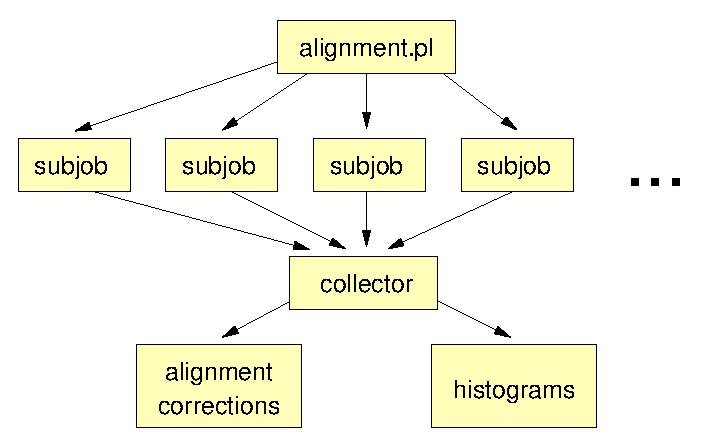
\includegraphics[width=0.8\linewidth]{flow}
\end{center}
\end{frame}

\begin{frame}
\frametitle{Existing Infrastructure in CommonAlignment*/HIP}
\begin{itemize}\setlength{\itemsep}{0.5 cm}
\item HIP algorithm is a weighted mean of residuals $\sum x_i w_i / \sum w_i$
\begin{enumerate}
\item $N$ subjobs calculate residuals over subsets of the data, saves
$\sum x_i w_i$ and $\sum w_i$ to job$N$/IOUserVariables.root
\item 1 collector job reads all job$N$/IOUserVariables.root, computes average.
\end{enumerate}
\item alignment.pl splits the data and submits subjobs to ``cmsalca''
farm; we can modify this for muon alignment
\item CommonAlignmentMonitor rides in the same job with HIPAlignmentAlgorithm
\begin{enumerate}
\item in a subjob, it saves histograms to job$N$/histograms.root
\item in a collector job, it reads all job$N$/histograms.root, and
merges them all (preserving directory structure)
\end{enumerate}
{\small (only histograms are merged, not ntuples)}
\end{itemize}
\end{frame}

%% \begin{frame}
%% \frametitle{Large(r) statistics test}
%% \begin{columns}
%% \column{0.6\linewidth}
%% Quarter million (12 GB AlCaReco) StandAlone muons from $Z\to\mu\mu$ processed in 2.75 hours on one computer: 1 mm resolution
%% \column{0.4\linewidth}
%% \mbox{\hspace{-0.2\linewidth} \includegraphics[width=1.2\linewidth]{quarter_million.png}}
%% \end{columns}

%% \vfill
%% \begin{itemize}\setlength{\itemsep}{0.5 cm}
%% \item Scaled to design resolution (250/150 $\mu$m DT/CSC): \\ 1 million muons in 11 hours
%% \item But $Z\to\mu\mu$ is especially clean: simple read-out of 500 QCD
%% events (tracker data) took 10 minutes: 30 times as long
%% \item Assume 330 computer-hours for 1 million muons: 3.3 hours on 100 computers
%% \end{itemize}
%% \end{frame}

\begin{frame}
\frametitle{Large(r) statistics test}
\begin{itemize}\setlength{\itemsep}{0.4 cm}
\item $\frac{1}{4}$ million StandAlone muons from $Z\to\mu\mu$ (12 GB AlCaReco) processed in \fbox{2.75 hours} on one computer
\item 1 mm $x$/1.6 cm $y$ alignment resolution--- assuming design resolution is 250 $\mu$m in $x$
\item Scaled to design resolution: 4 million StandAlone
muons or 0.04 million Global muons?  (10$\times$ better resolution)
\item But $Z\to\mu\mu$ is especially clean: simple read-out of 500 QCD
events (tracker tracks) took 10 minutes: \fbox{30 times as long}
\item 4 million StandAlone muons: 44 computer-hours/iteration \\
0.04 million Global muons: 13 computer-hours/iteration?
\end{itemize}
\end{frame}

\begin{frame}
\frametitle{CSA07 Logistics}
\begin{itemize}\setlength{\itemsep}{0.2 cm}
\item We'd like to run both algorithms: how does MuonStandAloneAlgorithm parallel-process?
\begin{enumerate}
\item Fill a matrix (ROOT file) in the loop over hits (Mille), and
\item invert the matrix in ROOT (Pede)?
\end{enumerate}
\item If so, we can put the matrix-filling part in the same event loop
as iteration 1 of HIPAlignmentAlgorithm (in $N$ subjobs)
\item HIPAlignmentAlgorithm/CommonAlignmentMonitor collection jobs
would be separate from the ROOT matrix inversion
\end{itemize}

\begin{itemize}\setlength{\itemsep}{0.2 cm}
\item Submit on ``cmsalca'' farm, use CASTOR for disk space?
\item HIPAlignmentAlgorithm disk space is dominated by histograms; is
MuonStandAloneAlgorithm disk space dominated by the matrix?
\end{itemize}
\label{numpages}
\end{frame}

\end{document}
